\documentclass{standalone}
\usepackage{tikz}

\usetikzlibrary{calc,shadows}


\begin{document}

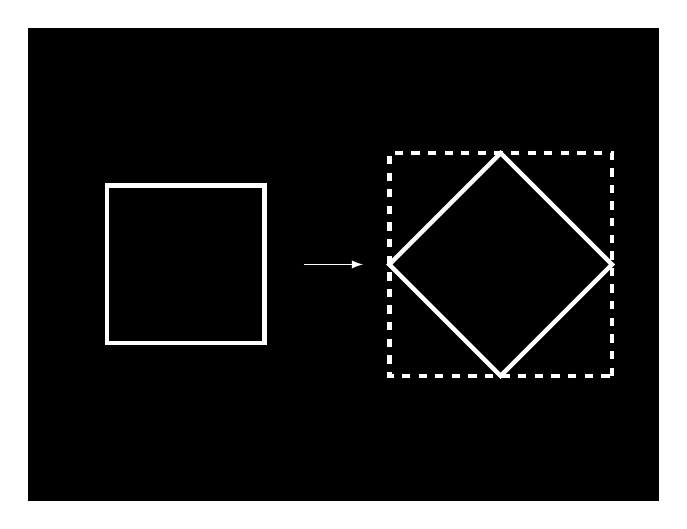
\begin{tikzpicture}
  \draw[fill=black,use as bounding box] (-4,-3) rectangle (4,3);

  \begin{scope}[xshift=-2cm]
    \draw[ultra thick,white] (-1,-1) rectangle (1,1);
  \end{scope}

  \begin{scope}[xshift=2cm]
    \begin{scope}[rotate=45]
      \coordinate (p1) at (-1,-1);
      \coordinate (p2) at (1,1);
      \coordinate (p3) at (-1,1);
      \coordinate (p4) at (1,-1);
      \draw[ultra thick,white] (p1) rectangle (p2);
    \end{scope}
    \draw let \p1=(p1), \p2=(p2), \p3=(p3), \p4=(p4) in
          [ultra thick,dashed,white] (\x4,\y1) rectangle (\x3,\y2);
  \end{scope}

  \draw[-latex,white] (-0.5,0) -- (0.25,0);
\end{tikzpicture}

\end{document}